\chapter{Conception}
%%%%%%%%%%%%%%%%%%%%%%%%%%%%%%%%%%%%%%%%%%%%%%%%%%%%%%
\section*{Introduction}
Ce chapitre est consacré, en premier lieu, à visualiser la conception générale de l'application en particulier son architecture logique. En deuxième lieu, nous présenterons l’enchaînement de conception qui a pour but de mieux expliciter les fonctionnalités en se basant sur les diagrammes de séquences. L’objectif recherché étant de façonner le système et de lui donner une forme répondant à tous les besoins et exigences recensés.
%%%%%%%%%%%%%%%%%%%%%%%%%%%%%%%%%%%%%%%%%%%%%%%%%%%%%%%
\section{Conception générale}
Dans cette section, nous présentons, en premier lieu, les interactions des composants de notre application dans un diagramme de déploiement. En deuxième lieu, nous exposons l'architecture logique ainsi que le diagramme de paquetage. 
%%%%%%%%%%%%%%%%%%%%%%%%%%%%%%%%%%%%%%%%%%%%%%%%%%%%%%
\subsection{Diagramme de déploiement de l'application}
La Figure \ref{fig:diagram_deploiement} décrit l'infrastructure selon laquelle notre application est déployée. Cette infrastructure est constituée des éléments suivants :
\begin{itemize}
    \item \textbf{Serveur web} : il contient un seul composant "Angular Frontend" qui est la partie forntend de notre application.
    \item \textbf{Serveur} : il contient plusieurs composants : 
    \begin{itemize}
        \item \textbf{Gateway}: c'est le composant qui est responsable de l'acheminement des requêtes reçues du serveur web vers les différents microservices, dont le module "Gestion Candidat".
        \item \textbf{Eureka discovery service}: c'est un service de découverte des microservices qui permet de signaler un microservice défectueux.
        \item \textbf{Configuration} : c'est le composant qui contient toute la configuration des différents microservices.
        \item \textbf{Gestion candidat} : c'est le microservice objet de ce travail qui est composé principalement de trois parties : 
        \begin{itemize}
            \item G\textbf{estion candidat Controller} : qui contient les différents web services REST.
            \item \textbf{Gestion candidat Service} : qui contient le métier de notre module.
            \item \textbf{Gestion candidat DAO} : qui contient la partie de persistance des données dans la base de données.
        \end{itemize}
    \end{itemize}
    \item \textbf{Serveur Base de données} : il contient un seul composant, qui est le Système de gestion de base de données Postgresql.
\end{itemize}
\begin{figure}[H]
     \centering
     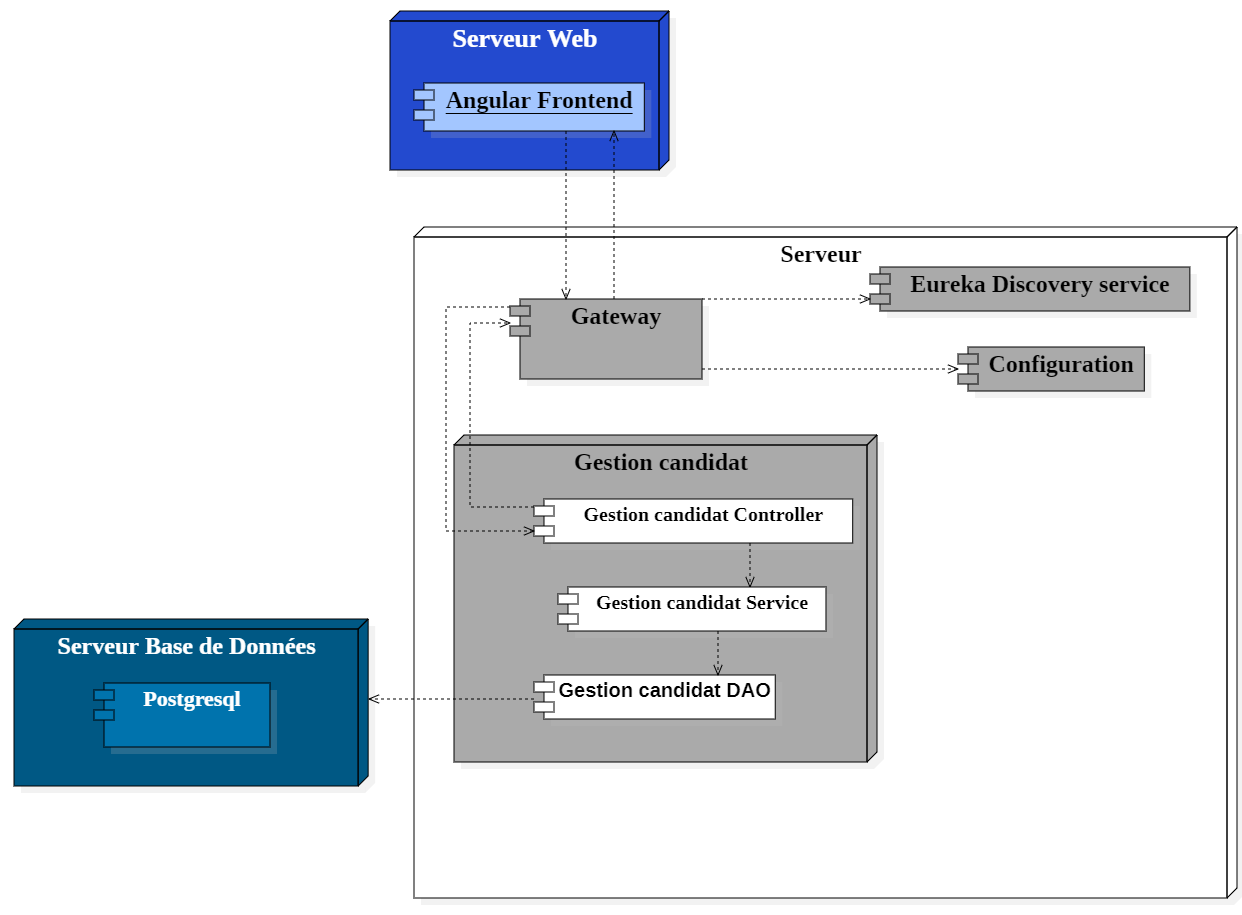
\includegraphics[scale=0.5]{img/DeploymentDiagram1.png}
     \caption{Diagramme de déploiement de l'application}
     \label{fig:diagram_deploiement}
 \end{figure}
%%%%%%%%%%%%%%%%%%%%%%%%%%%%%%%%%%%%%%%%%%%%%%%%%%%%%%
 \subsection{Architecture logique de l'application}
 L’architecture logique décrit les différentes couches d’une application, leurs interrelations et leurs interactions. Notre module de gestion des candidats est composé des couches suivantes présentées dans la Figure \ref{fig:archi_logique}.
 \begin{itemize}
     \item \textbf{Couche présentation} : cette couche contient les interfaces graphiques qui permettent la visualisation des données pour l'utilisateur.
     \item \textbf{Couche contrôleur} : cette couche contient les différents web services REST qui permettent de relier la couche présentation avec la partie métier de notre application.
     \item \textbf{Couche Service} : cette couche contient les différents services métier de l'application.
     \item \textbf{Couche Mapper} : cette couche permet la transformation des objets sous forme DTO (provenant de la couche présentation) en des entités.
     \item \textbf{Couche persistance} : cette couche permet l'interaction avec la base de données pour ajouter, modifier, supprimer ou bien consulter des données.
 \end{itemize}
 \begin{figure}[H]
     \centering
     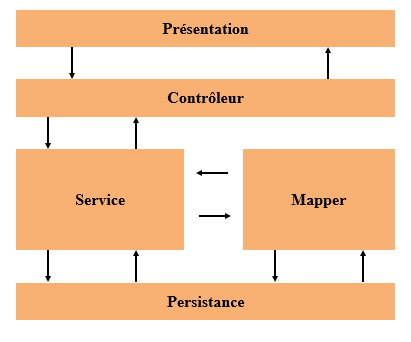
\includegraphics[scale=1]{img/archi logique.PNG}
     \caption{Architecture logique du module de gestion des candidats}
     \label{fig:archi_logique}
 \end{figure}
 %%%%%%%%%%%%%%%%%%%%%%%%%%%%%%%%%%%%%%%%%%%%%%%%%%%
 \subsection{Diagramme de paquetage}
 Notre application doit garantir une indépendance dans les rôles entre ses différents modules qui sont représentés dans la Figure \ref{fig:diagram_package} :
 \begin{itemize}
     \item Le paquetage \textbf{Controller} contient les web services REST.
     \item Le paquetage \textbf{Dto} contient les différentes classes Dto qui représentent les objets envoyés et reçus de la partie frontend.
     \item Le paquetage \textbf{Services} contient les différentes classes de la logique métier.
     \item Le paquetage \textbf{Mapper} contient les différentes classes qui permettent la transformation des objets Dto en des entités pour les enregistrer, les modifier ou les supprimer de la base de données.
     \item Le paquetage \textbf{Dao} contient les différentes interfaces contenant les méthodes qui permettent la persistance des données dans la base de données.
     \item Le paquetage \textbf{Entities} contient les différentes classes des entités relatives aux tables de la base de données.
 \end{itemize}
  \begin{figure}[H]
     \centering
     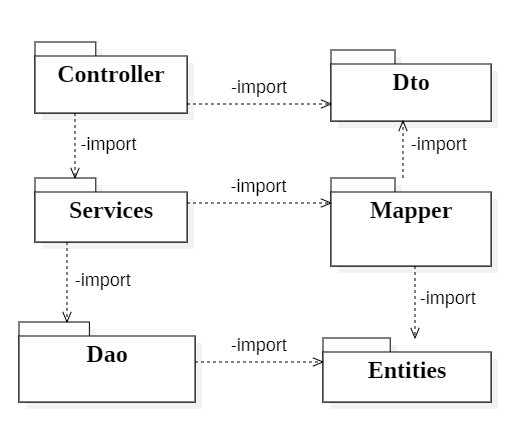
\includegraphics[scale=0.8]{img/Package Diagram.png}
     \caption{Diagramme de paquetage}
     \label{fig:diagram_package}
 \end{figure}
 %%%%%%%%%%%%%%%%%%%%%%%%%%%%%%%%%%%%%%%%%%%%%%%%%%%
\section{Conception détaillée}
Après avoir précisé les différents aspects de la conception générale de notre application, nous passons à la conception détaillée. Dans cette section, nous présentons le diagramme de classe ainsi que les diagrammes de séquences.
\subsection{Diagramme de classes}
Les diagrammes de classes sont l'un des types de diagrammes les plus utiles, car ils décrivent clairement la structure d’un système particulier en modélisant ses classes, ses attributs, ses opérations et les relations entre ses objets. La Figure \ref{fig:diagram_class} représente le diagramme de classes relatif à notre application.
 \begin{figure}[H]
     \centering
     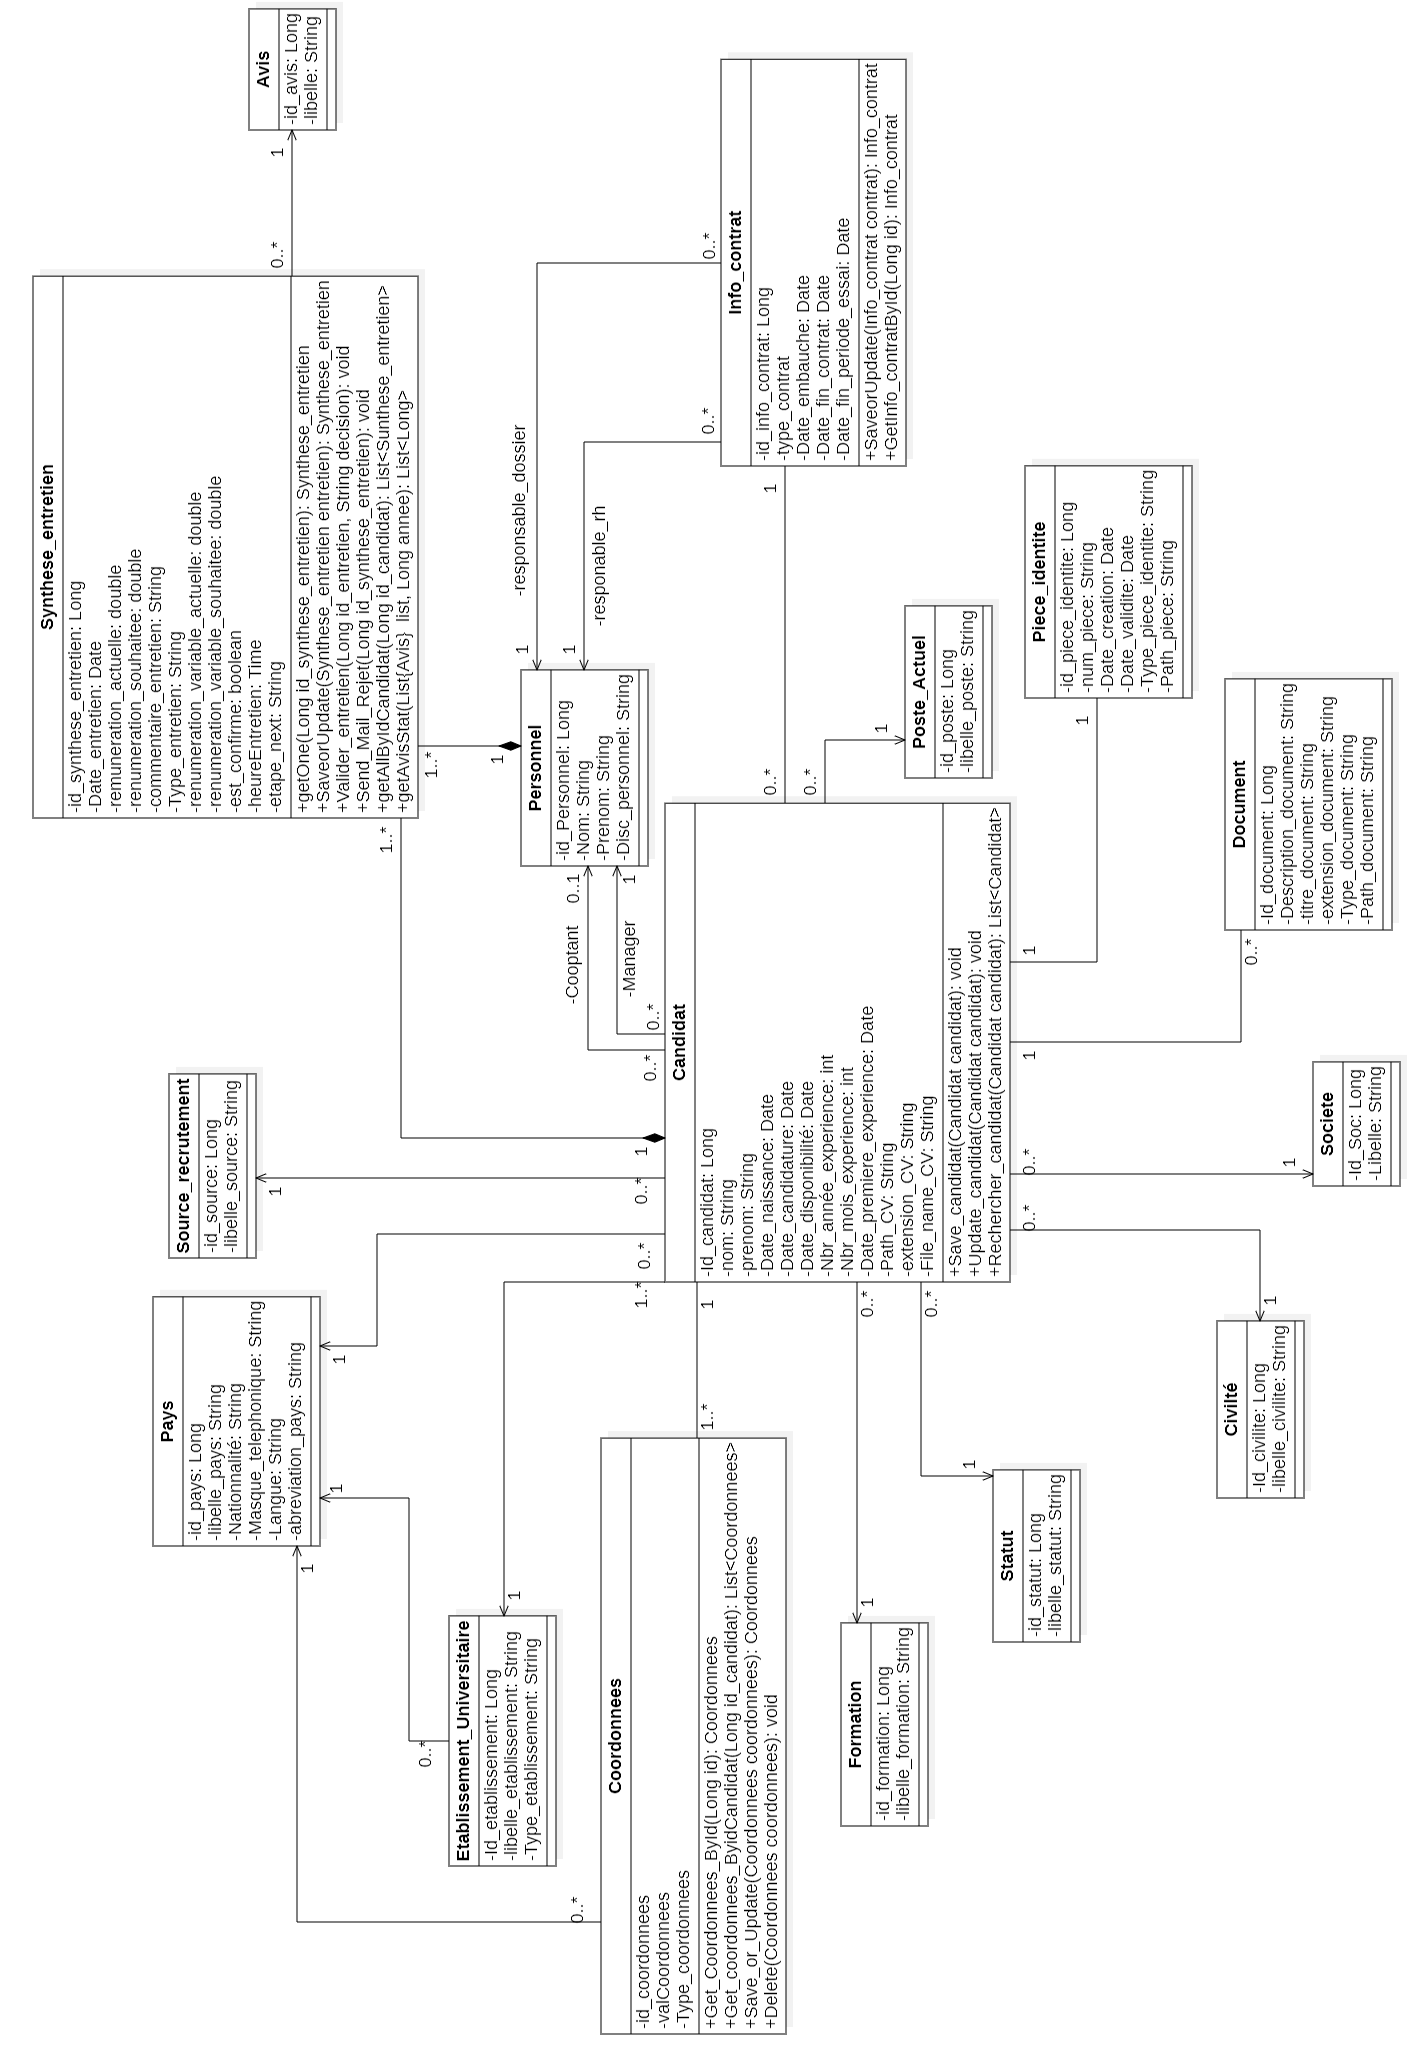
\includegraphics[scale=0.45]{img/ClassDiagram2.png}
     \caption{Diagramme de classes}
     \label{fig:diagram_class}
 \end{figure}
\newpage
Le diagramme représenté par la Figure \ref{fig:diagram_class} est constitué des classes suivantes:
\begin{itemize}
    \item \textbf{Classe coordonnées} : cette classe permet de gérer les coordonnées relatives à un candidat (un e-mail ou bien un numéro de téléphone).
    \item \textbf{Classe Info\_contrat} : cette classe permet de gérer les informations concernant le contrat (salaire, durée,poste, régime\dots) à signer par candidat s'il sera accepté.
    \item \textbf{Classe Synthese\_entretien} : cette classe permet de gérer les entretiens du candidat.
    \item \textbf{ Classe Candidat} : cette classe permet de gérer la fiche du candidat.
    
\end{itemize}
\subsection{Diagrammes de séquences}
Les diagrammes de séquences sont la représentation graphique des interactions entre les acteurs et le système selon un ordre chronologique. Dans cette partie, nous présentons les principaux diagrammes de séquences relatifs aux fonctionnalités de notre application.
\subsubsection{Ajouter une fiche candidat}
La Figure \ref{fig:sequence_ajout_fiche} représente le diagramme de séquence relatif à l'ajout d'une nouvelle fiche candidat. 
 \begin{figure}[H]
     \centering
     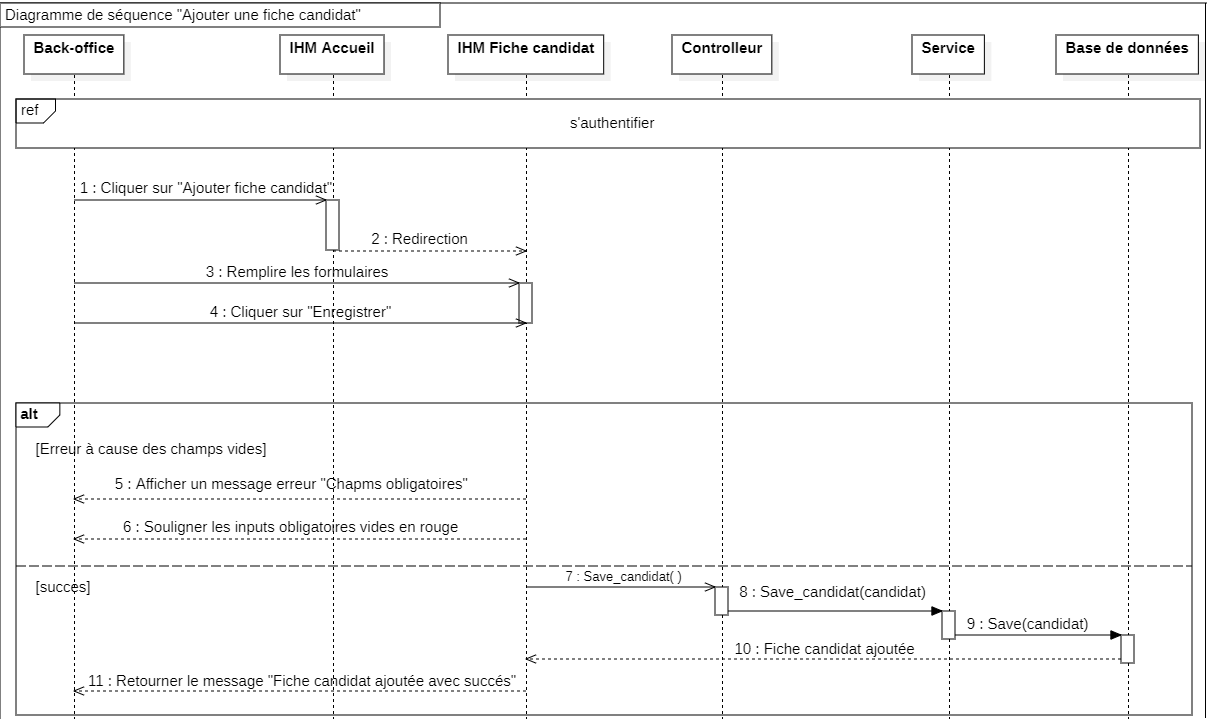
\includegraphics[scale=0.51]{img/sequence ajouter fiche candidat.png}
     \caption{Diagramme de séquence "Ajouter une fiche candidat"}
     \label{fig:sequence_ajout_fiche}
 \end{figure}
 Le back-office doit s'authentifier pour accéder à l'interface de la fiche candidat en cliquant sur "Ajouter fiche candidat" à partir de l'interface d'accueil. Il doit ensuite remplir le formulaire de la fiche et cliquer sur "Enregistrer". Un objet candidat est envoyé au contrôleur qui le passe, à son tour, au service pour l'enregistrer dans la base de données.
 %%%%%%%%%%%%%%%%%%%%%%%%%%%%%%%%%%%%%%%%%%%%%
 \subsubsection{Rechercher un candidat}
 Le diagramme de séquence du cas d'utilisation "Rechercher un candidat" est représenté par la Figure \ref{fig:sequence_recherche_candidat}
  \begin{figure}[H]
     \centering
     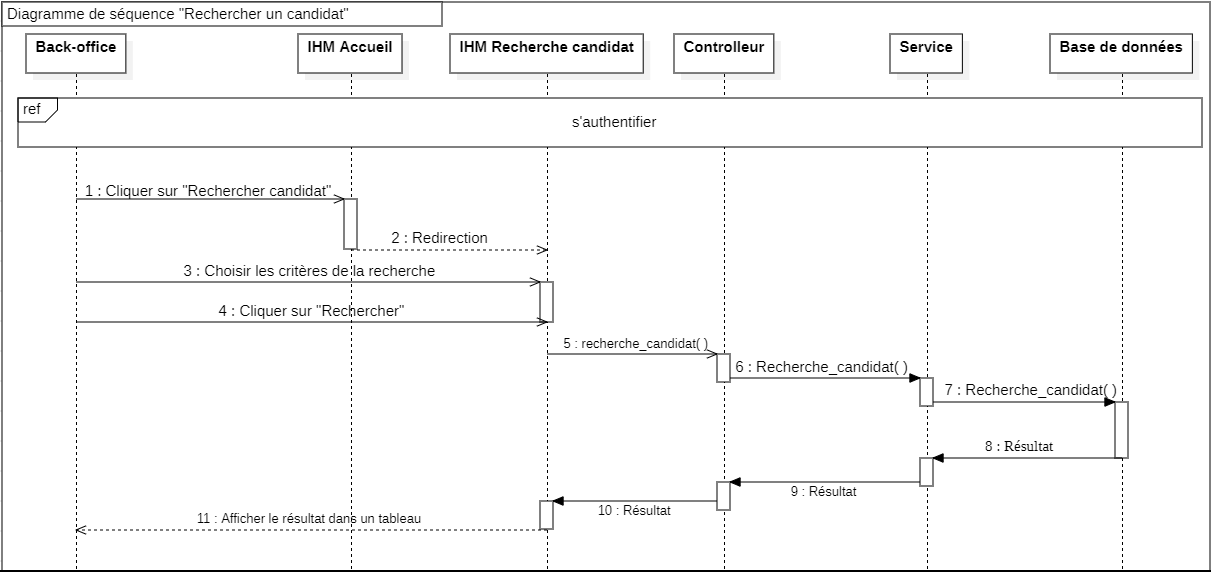
\includegraphics[scale=0.51]{img/sequence recherche candidat.png}
     \caption{Diagramme de séquence "Rechercher un candidat"}
     \label{fig:sequence_recherche_candidat}
 \end{figure}
 Après authentification, le back-office clique sur le bouton "Rechercher un candidat". Une fois l'interface de la recherche est chargée, le back-office choisit les critères de recherche(liste déroulante,case à cocher$\dots$) et clique sur le bouton "Rechercher". Un objet contenant les critères de recherche est envoyé au contrôleur, puis passé au service afin d'exécuter la méthode de la recherche. Le résultat est envoyé sous forme d'une liste des candidats à l'interface de la recherche où le résultat est affiché sous forme d'un tableau. Chaque ligne du tableau contient quelques informations qui concernent le candidat ainsi qu'un bouton pour consulter la fiche du candidat. 
 %\newpage
 %%%%%%%%%%%%%%%%%%%%%%%%%%%%%%%%%%%%%%%%%%%%%%%%%
 \subsubsection{Planifier un entretien}
 La Figure \ref{fig:sequence_planifier_entretien} illustre le diagramme de séquence relatif à la planification d'un nouvel entretien.
 \newpage
 \begin{figure}[H]
     \centering
     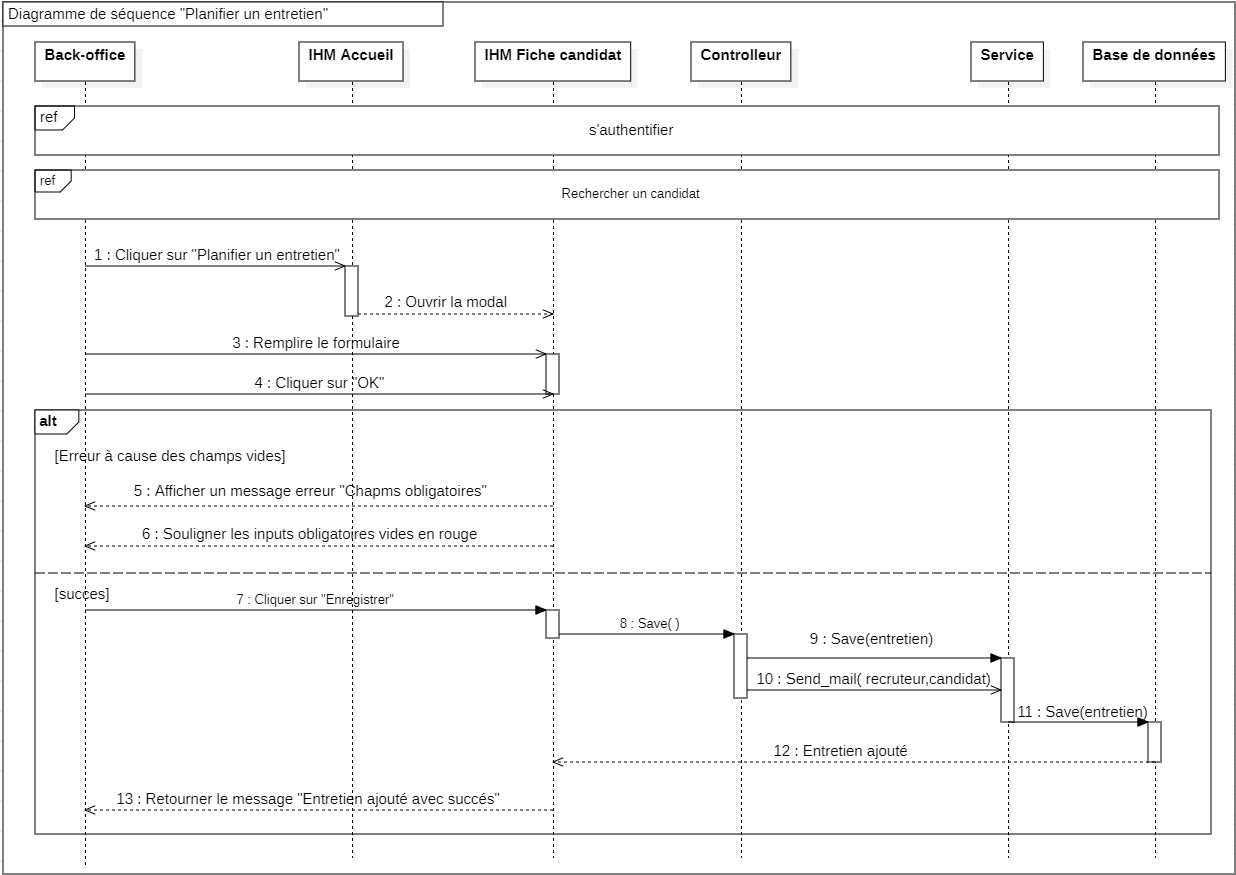
\includegraphics[scale=0.51]{img/sequence planifier entretien.png}
     \caption{Diagramme de séquence "Planifier un entretien"}
     \label{fig:sequence_planifier_entretien}
 \end{figure}
 Une fois le back-office s'est authentifié et a effectué une recherche, il planifie un nouvel entretien en cliquant sur le bouton "Planifier un entretien". Après, il remplit le formulaire et clique sur "OK". Le système vérifie qu'il n'y a pas des champs obligatoires vides et enregistre l'entretien. Enfin, un e-mail est envoyé pour  notifier le recruteur sélectionné lors de la planification de l'entretien.
 %%%%%%%%%%%%%%%%%%%%%%%%%%%%%%%%%%%%%%%%%%%%%%%%%
 \subsubsection{Accepter un entretien}
 Le diagramme de séquence relatif au cas d'utilisation "Accepter un entretien" est représenté dans la Figure \ref{fig:sequence_accepter_entretien}.
 \begin{figure}[H]
     \centering
     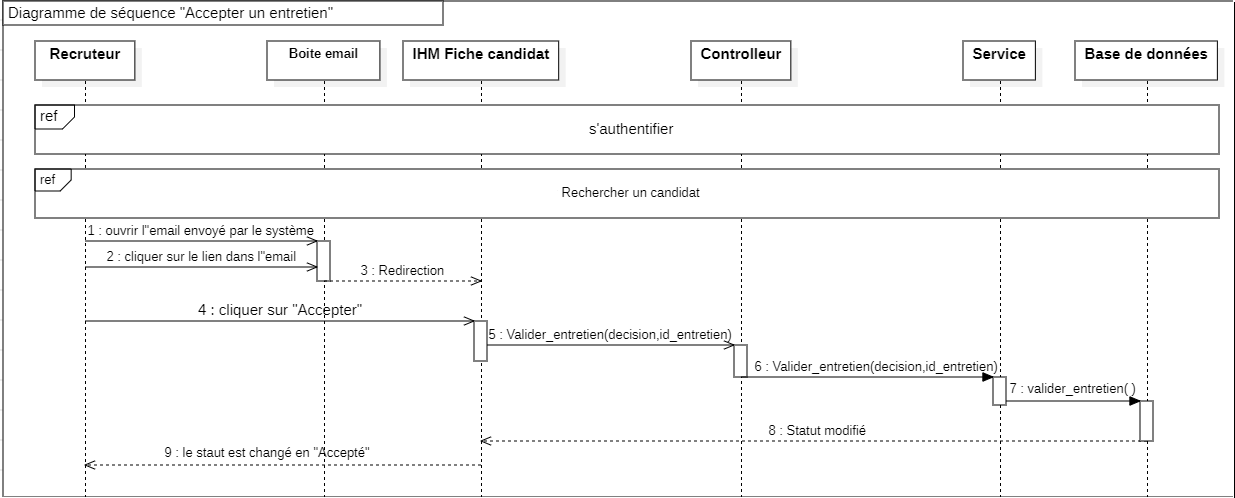
\includegraphics[scale=0.51]{img/sequence accepter entretien.png}
     \caption{Diagramme de séquence "Accepter un entretien"}
     \label{fig:sequence_accepter_entretien}
 \end{figure}
 Une fois un entretien est planifié, le recruteur consulte l'e-mail reçu dans son courrier électronique et contenant les informations relatives à l'entretien. Il clique alors sur le lien qui lui est envoyé dans l'e-mail et qui le redirige vers la fiche du candidat. Il clique sur le bouton "Accepter", ce qui modifie le statut de l'entretien en "Accepté".
 %%%%%%%%%%%%%%%%%%%%%%%%%%%%%%%%%%%%%%%%%%%%%%%%%%%
 \subsubsection{Rejeter un entretien}
 La Figure \ref{fig:sequence_refuser_entretien} représente le diagramme de séquence relatif au cas d'utilisation "Rejeter un entretien".
 \begin{figure}[H]
     \centering
     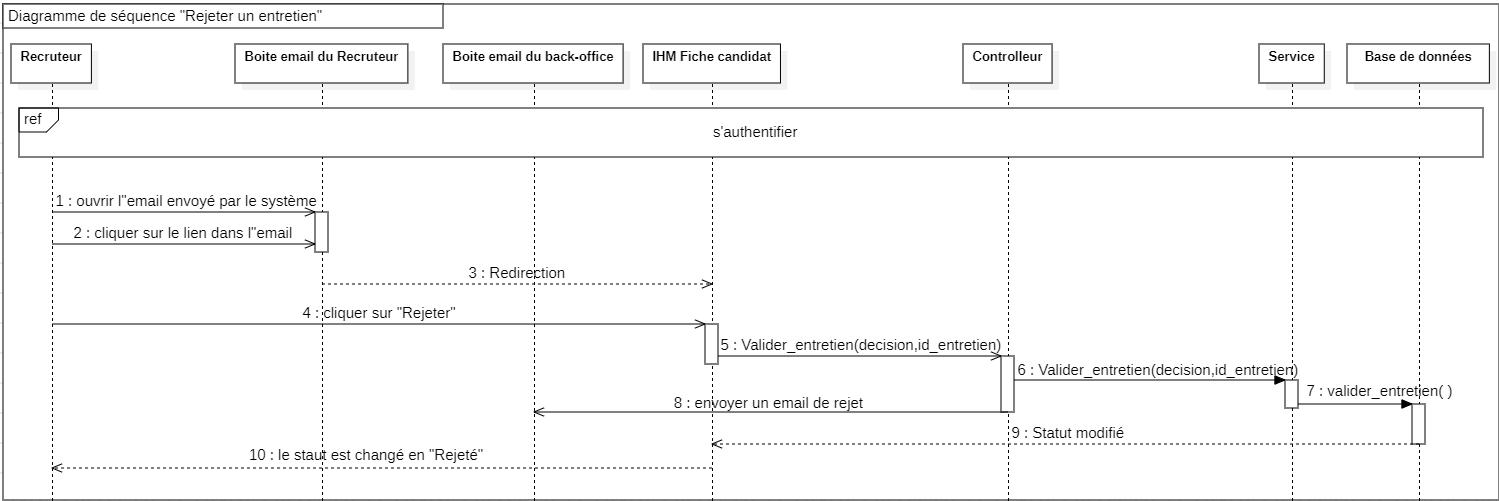
\includegraphics[scale=0.4]{img/sequence refuser entretien.png}
     \caption{Diagramme de séquence "Rejeter un entretien"}
     \label{fig:sequence_refuser_entretien}
 \end{figure}
   Une fois un entretien est planifié, le recruteur consulte l'e-mail reçu dans son courrier électronique et contenant les informations relatives à l'entretien. Il clique alors sur le lien qui lui est envoyé dans l'e-mail et qui le redirige vers la fiche du candidat. Il clique sur le bouton "Rejeter", un e-mail est alors envoyé au back-office pour le notifier du rejet de l'entretien par le recruteur. Ainsi, le statut de l'entretien est modifié en "Rejeté".
  %%%%%%%%%%%%%%%%%%%%%%%%%%%%%%%%%%%%%%%%%%%%%%%%%%%%
 \subsubsection{Modifier une fiche candidat}
 Le diagramme de séquence relatif à la modification d'une fiche candidat est représenté dans la Figure \ref{fig:sequence_modif_fiche}.
 \begin{figure}[H]
 \centering
 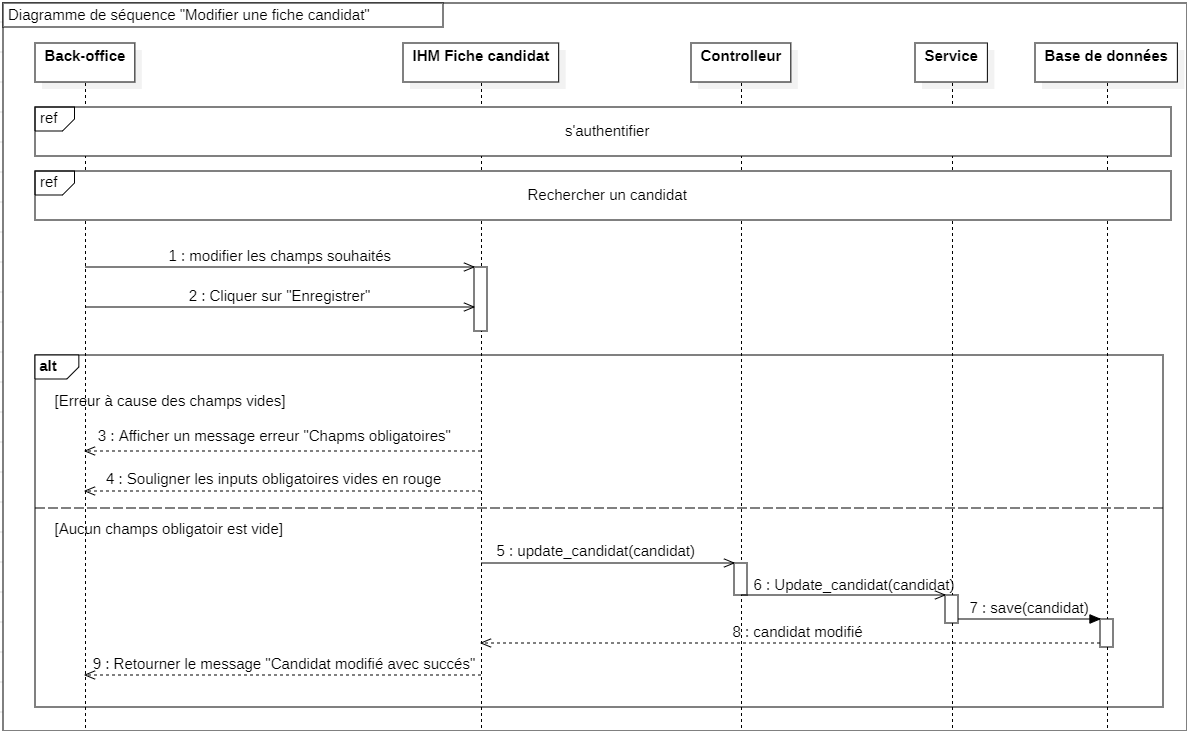
\includegraphics[scale=0.51]{img/sequence modifier fiche candidat.png}
 \caption{Diagramme de séquence "Modifier une fiche candidat"}
 \label{fig:sequence_modif_fiche}
 \end{figure}
 Après son authentification, et la recherche de la fiche d'un candidat, le back-office procède au modifications de champs qu'il juge nécessaires dans le formulaire affiché, puis clique sur le bouton "Enregistrer". Le système vérifie que les champs obligatoires sont remplis et enregistre les modifications. Enfin, un message contenant "Candidat modifié avec succès" est affiché.
 %%%%%%%%%%%%%%%%%%%%%%%%%%%%%%%%%%%%%%%%%%%%%%%%%%%%%%
\section*{Conclusion}
Dans le présent chapitre, nous avons présenté la conception générale de notre application. Par la suite, nous avons passé en revue la conception détaillée, en enchaînant par le diagramme de classes ainsi que les diagrammes de séquences pour mieux visualiser l'interaction des acteurs avec le système.
Dans le prochain chapitre, nous allons montrer comment nous avons traduit cette étude conceptuelle et à l’aide de quels outils nous avons pu mettre en place notre application.
